\title{Experimental Laboratory 3\\Analysis of the hydrodynamic forces acting on a cylinder in steady free surface flow}
\author{
        Sergio M. Vanegas A.\\
        Francesco de Pas\\
                Department of Mathematics\\
        Polimi---Politecnico di Milano\\
        Milano, Italia
}
\date{\today}

\documentclass[12pt]{article}

\usepackage{amsmath}
\usepackage{graphicx}
\usepackage{siunitx}

\begin{document}
\maketitle

\begin{abstract}

        Goal of this test case is to investigate the drag and lift forces acting on a cylinder submerged in a steady-state free-surface water flow. The experiments have been performed in the water channel facility of the Hydraulics Laboratory, and the two force components (horizontal and vertical) have been measured through a balance. In the case study proposed, the Reynolds number of the cylinder $Re=DU_\infty/\nu$ is within the range of the “sub-critical regime”\footnote{Note that the classification of flow regimes discussed in the class lecture refers to unconfined flows. This is not the case of this experiment, in which the cylinder is located in a water channel with finite size cross section. However, it is reasonable to expect some similar behavior to the unconfined case.}; therefore, it will be not surprising to notice that the flow separates at a certain distance from the front stagnation point, causing a recirculation zone behind it, and that an oscillating wake is created by the shedding of two counter-rotating vortexes. As a result, also drag and lift will show an oscillating behavior.\cite{FL:07}

\end{abstract}

\section{Introduction}

        The scheme of the experiment is reported in Figure~\ref{fig:reference} here below. The balance is fixed to the ground and connected to the cylinder through the endplates. The hydrodynamically shaped endplates allow to hold the cylinder and ensure some sort of “two-dimensional flow” around it by suppressing the three-dimensional effects at the cylinder ends. Two load cells are installed inside the balance, one for measuring the horizontal force and the other for measuring the vertical force. The load cells provide an output voltage, which is linearly proportional to the applied force.

        \begin{figure}[ht!]
                \centering
                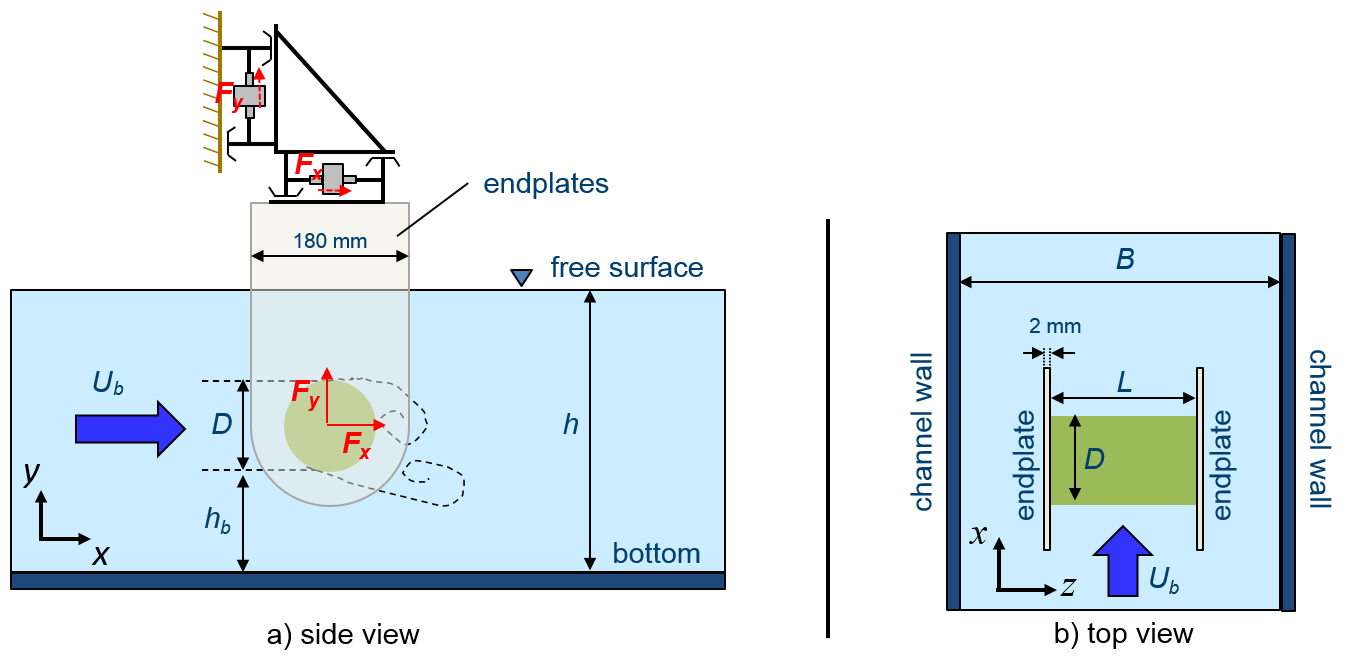
\includegraphics[width=\textwidth]{Setup.png}
                \caption{Sketch of the experiment}
                \label{fig:reference}
        \end{figure}

        The calibration of the balance has been performed after the installation of the endplates and the cylinder on the balance, by applying weight standards to the cylinder without water in the channel. When developing the calibration function, it was taken into account that the real forces experienced by the cells are not only those produced by the applied load, but they also include the weight of the structure, and other small contributions related with the deformability of the structure. The calibration function has been determined in such a way that the condition $F_x=0$, $F_y=0$ corresponds to the absence of applied (external) forces, net of the weight and the small deformability-related contributions.

        When water flows in the channel, assuming that the dynamic forces on the endplates is negligible since they are hydrodynamically shaped, the horizontal external force $F_x$ is equal to the drag force acting on the cylinder, $F_D$. Conversely, the vertical external force $F_y$ is equal to the sum of the lift force acting on the cylinder $F_L$ and the buoyancy force acting on the cylinder and the endplates, $F_B$. Thus, whereas $F_D$ is simply taken as the calibration output $F_x$, $F_L$ will be given as $F_y - F_B$. The buoyancy force, $F_B$, could be theoretically calculated by multiplying the volume of the immersed parts (cylinder and part of the endplates) by the specific weight of water. However, since knowing all the geometrical details with high accuracy is not trivial, directly measuring $F_B$ with the balance appears a preferred option. This is achieved by making a test in still water with the same level of the flowing-water test. Since no drag and lift forces play a role in the static test, in this case the horizontal external force $F_x$ will be zero and the vertical external force $F_y$ will be equal to $F_B$.

        The input data of the problem is summarized in Table~\ref{tab:input_data}.

        \begin{table}[ht!]
                \centering
                \begin{tabular}{llll}
                        \hline
                        \textbf{Symbol}     & \textbf{Parameter}        & \textbf{Value}        & \textbf{Units}        \\ \hline
                        \textit{B}      & Width of the channel  & 0.5   & m     \\
                        \textit{D}      & Diameter of the Cylinder      & 0.06  & m     \\
                        \textit{L}      & Width of the Cylinder & 0.185 & m     \\
                        \textit{t}      & Thickness of the endplates    & 0.002 & m     \\
                        \textit{b}      & Length of the endplates       & 0.180 & m     \\
                        \textit{h}      & \begin{tabular}[c]{@{}l@{}}Water level in the channel\\ upstream of the cylinder\end{tabular} & 0.45  & m     \\
                        \textit{$h_b$}    & \begin{tabular}[c]{@{}l@{}}Distance of the cylinder wall\\ from the channel bottom\end{tabular}      & 0.18 & m     \\
                        $f_s$   & Sampling frequency    & 200   & Hz    \\
                        \textit{Q}       & Volumetric flow rate of water & 75    & L/s   \\
                        \textit{$\rho$} & Density of water  & 998   & $\text{Kg}/m^3$       \\
                        \textit{$\mu$}   & Dynamic viscosity of water    & 0.001 & Pa$\cdot$s  \\ \hline
                \end{tabular}
                \caption{Input Data}
                \label{tab:input_data}
        \end{table}

        The complete set of acquisition data is provided in the MATLAB\\ workspaces from Table~\ref{tab:workspace}. In each workspace, the values of $F_x$ and $F_y$ are provided in the form of vectors. These values have already been converted from the voltage output of the cells through the calibration functions, as explained previously.

        \begin{table}[ht!]
                \centering
                \begin{tabular}{|l|l|}
                        \hline
                        \textbf{Filename}       & \textbf{Condition}    \\ \hline
                        \texttt{FORCEdata\_nowater.mat}  & \begin{tabular}[c]{@{}l@{}}Cylinder and endplates, no water in the\\ channel\end{tabular}     \\ \hline
                        \texttt{FORCEdata\_stillwater.mat} & \begin{tabular}[c]{@{}l@{}}Cylinder and endplates, still water in the\\ channel\end{tabular}        \\ \hline
                        \texttt{FORCEdata\_flow.mat}       & \begin{tabular}[c]{@{}l@{}}Cylinder and endplates, flowing water in\\ the channel\end{tabular}      \\ \hline
                        \texttt{FORCEdata\_NatOsc.mat} & \begin{tabular}[c]{@{}l@{}}Cylinder and endplates, still water in the\\ channel, cylinder hit once manually\end{tabular}        \\ \hline
                \end{tabular}
                \caption{MATLAB workspace descriptions}
                \label{tab:workspace}
        \end{table}
        
        The remainder of the report is organized as follows: in Section~\ref{sec:setup}, we approximate the channel Bulk velocity, the setup's Reynolds number and the Buoyancy Force, which will be fundamental for the analysis of the experimental data; in Section~\ref{sec:static} we analyze the Reynolds-Averaged Forces and Coefficients, as well as its measurement error; in Section~\ref{sec:dynamic} we identify the vortex shedding frequency and compare it to the natural frequencies of the balance structure in still water; finally, in Section~\ref{sec:optional} we further analyze the oscillations of the Lift Force and the hypothetical error induced by a variation in the setup's water level.

\section{Parameter Acquisition} \label{sec:setup}

        Since the experiments involve a water flow in a finite size channel, $ U_b \neq U_\infty $; nevertheless, it is a reasonable first approximation for our case of study. We approximate the channel bulk velocity through the expression in Equation~\ref{eq:Ub}. Then, we use this value to approximate the Reynolds number as in Equation~\ref{eq:Re}.

        \begin{equation} \label{eq:Ub}
                U_b = \frac{Q}{B h} = \SI{3.333E-1}{\metre \per \second}
        \end{equation}

        \begin{equation} \label{eq:Re}
                \text{Re} = \frac{D U_\infty}{\nu} \approx \frac{D U_b}{\nu} = \num{1.996E4}
        \end{equation}

        Using the data from \texttt{FORCEdata stillwater.mat}, we averaged the vertical force registered by the sensor when there is no flow, which corresponds to the buoyancy force exerted by the medium: \SI{7.325E0}{\newton}. This value will be subtracted from the registered force from now on in order to get the real value of the force exerted by the flow along the vertical axis.

\section{Reynolds-Averaged Analysis} \label{sec:static}

        We then loaded \texttt{FORCEdata\_flow.mat} and averaged the data over time in order to get the Reynolds-Averaged value of the forces along x and y (\SI{9.157E-1}{\newton} and \SI{-2.181E-2}{\newton} respectively). Normalizing these values with the formula in Equation~\ref{eq:coeff}, we get the Reynolds-averaged Drag and Lift Coefficients (\num{1.488E0} and \num{-3.543E-2} respectively).

        \begin{equation} \label{eq:coeff}
                C_{D,L} = \frac{F_{D,L}}{\frac{1}{2} \rho A U_b^2} , A=LD
        \end{equation}

        In order to determine the uncertainty of the above coefficients, we made use of the \textit{Error-Propagation Law}: let $y=y(x_1,x_2,\dots,x_n)$ be the quantity of interest; then, the uncertainty $u(y)$ can be estimated as $$u(y) = \sqrt{\left(\frac{\partial y}{\partial x_1} u(x_1)\right)^2 + \left(\frac{\partial y}{\partial x_2} u(x_2)\right)^2 + \dots + \left(\frac{\partial y}{\partial x_n} u(x_n)\right)^2}$$

        In our specific case, we can estimate the uncertainties of interest as in Equation~\ref{eq:uncertainty}, particularly the uncertainties of the Drag and Lift coefficients (\num{9.229E-2} and \num{4.064E-2} respectively). It is worth noting that the Lift coefficient uncertainty is comparable to its magnitude, meaning that the expected 0 average value is well within the estimation's interval of accuracy. On the other hand, the Drag coefficient uncertainty is two order of magnitude below its magnitude, meaning that we can rely on the calculated value.

        \begin{align} \label{eq:uncertainty}
                \begin{cases}
                        u(A) &= \sqrt{\left(D u(L)\right)^2 + \left( L u(D) \right)^2}\\
                        u(U_b) &= \sqrt{\left(\frac{1}{B h} u(Q)\right)^2 + \left(\frac{-Q}{B^2 h} u(B)\right)^2 + \left(\frac{-Q}{B h^2} u(h)\right)^2}\\
                        u(C_{D,L}) &= \sqrt{\left(\frac{1}{\frac{1}{2} \rho A U_b^2} u(F_{D,L})\right)^2 + \left(\frac{-F_{D,L}}{\frac{1}{2} \rho A^2 U_b^2} u(A)\right)^2 \left(\frac{-2 F_{D,L}}{\frac{1}{2} \rho A U_b^3} u(U_b)\right)^2}
                \end{cases}
        \end{align}

\section{Dynamic Analysis} \label{sec:dynamic}

        Once we were done with the static analysis, we loaded both \texttt{FORCEdata flow.mat} and \texttt{FORCEdata NatOsc.mat}. We then applied an FFT to both datasets' Vertical Force and extracted the highest peak's frequency location, revealing that the Vortex-shedding frequency and Natural oscillation frequency were \SI{1.008E0}{\hertz} and \SI{3.126E-2}{\hertz} respectively. As we can clearly notice, these values are 2 orders of magnitude apart from each other, making it clear that the oscillations we register during the flow correspond to the Vortex-shedding characteristic frequency instead of a natural resonance.

\section{Optional Questions} \label{sec:optional}

        After obtaining the characteristic frequencies of the system, we wanted to determine the amplitude of the flow oscillations along the vertical axis; in order to do this, a noise-free signal (or at least a high SNR) was required.
        
        We first filtered the data from the \texttt{FORCEdata flow.mat} dataset using a Low-Pass filter with a cutoff frequency of double the Vortex-shedding one; a comparison can be observed in Figure~\ref{fig:filtered}.

        \begin{figure}[ht!]
                \centering
                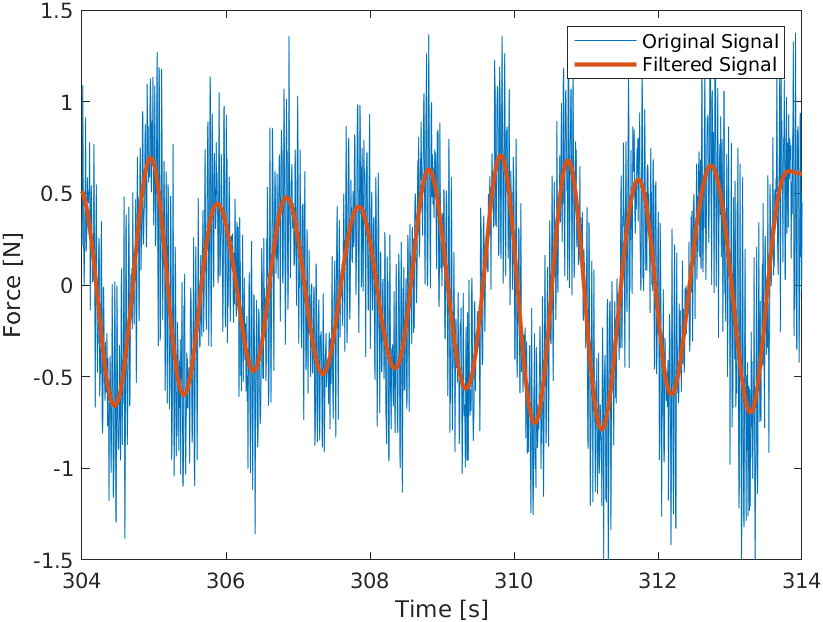
\includegraphics[width=\textwidth]{Filtered.png}
                \caption{Original signal vs Filtered signal}
                \label{fig:filtered}
        \end{figure}

        With the filtered signal, we extracted the amplitude using 2 different methods:

        \begin{itemize}
                \item Half the difference between the averaged maxima and minima ($a_\text{peak} = \SI{4.732E-1}{\newton}$).
                \item $\sqrt{2}$ times the RMS value of the signal ($a_\text{RMS} = \SI{5.198E-1}{\newton}$).
        \end{itemize}

        Using these values, we calculated the Fluctuating Lift coefficient as in Equation~\ref{eq:lift_p}, yielding $\num{7.689E-1}$ and $\num{8.446E-1}$ respectively. Regardless of the method, it is worth noting that this quantity is one order of magnitude above the Reynolds-averaged Lift coefficient, which is coherent with the studied theory.

        \begin{equation} \label{eq:lift_p}
                C_L' = \frac{a_L}{\frac{1}{2} \rho A U_\infty^2}
        \end{equation}

        Regarding the hypothetical errors, we first calculated the difference in Buoyancy Force induced by the bigger endplate portion of mass submerged resulting from the proposed water level variation as in Equation~\ref{eq:dFB}. Adding this value to the previously registered Force, we repeated the calculations for the Reynolds-averaged Drag and Lift coefficients and for the Fluctuating Lift coefficient and compared it to the original values. As expected, the Static Drag coefficient does not change at all, since the effect of the water level variation only has an effect along the vertical axis. Nevertheless, for this very reason both the Static and Fluctuating\footnote{Only if the RMS method is used.} Lift coefficients suffer a variation of 64\% and 0.2\% respectively. Such a high relative error in Static lift coefficient is due to the fact that a 0 average value for the vertical force is expected once the Buoyancy Force has been subtracted, instead for the fluctuating one, since no new fluctuation stimula are inserted, it is reasonable it remains almost the same.

        \begin{equation} \label{eq:dFB}
                \Delta F_B = - (2 t b) \rho g \Delta h \; , \; \Delta h = \SI{2E-3}{\metre}
        \end{equation}

\bibliographystyle{abbrv}
\bibliography{main}

\end{document}
